\appendices

\section{Github REST API Example}
\label{a-ghrest}

There are some API's calling examples.


\subsection{Get All Followers of a User}

\begin{minted}[breaklines,breakautoindent,mathescape,linenos,numbersep=1pt,frame=lines,framesep=2mm,fontsize=\footnotesize,baselinestretch =1,style=emacs]{python}
https://api.github.com/users/mateiz/followers
\end{minted}


\begin{minted}[breaklines,breakautoindent,mathescape,linenos,numbersep=1pt,frame=lines,framesep=2mm,fontsize=\footnotesize,baselinestretch =1,style=emacs]{json}
[
    {
        "login": "bennettandrews",
        "id": 1143,
        "node_id": "MDQ6VXNlcjExNDM=",
        "gravatar_id": "",
        "html_url": "https://github.com/bennettandrews",
        ...
    },
    ...
]
\end{minted}


\subsection{Get Repository's Detailed Information}

\begin{minted}[breaklines,breakautoindent,mathescape,linenos,numbersep=1pt,frame=lines,framesep=2mm,fontsize=\footnotesize,baselinestretch =1,style=emacs]{python}
https://api.github.com/repos/apache/spark
\end{minted}


\begin{minted}[breaklines,breakautoindent,mathescape,linenos,numbersep=1pt,frame=lines,framesep=2mm,fontsize=\footnotesize,baselinestretch =1,style=emacs]{json}
{
    "id": 17165658,
    "node_id": "MDEwOlJlcG9zaXRvcnkxNzE2NTY1OA==",
    "name": "spark",
    "full_name": "apache/spark",
    "private": false,
    "owner": {
        "login": "apache",
        "id": 47359,
        ...
    }
    ...
}
\end{minted}



\subsection{Get All Commits of a Repository}

\begin{minted}[breaklines,breakautoindent,mathescape,linenos,numbersep=1pt,frame=lines,framesep=2mm,fontsize=\footnotesize,baselinestretch =1,style=emacs]{python}
https://api.github.com/repos/apache/spark/commits
\end{minted}


\begin{minted}[breaklines,breakautoindent,mathescape,linenos,numbersep=1pt,frame=lines,framesep=2mm,fontsize=\footnotesize,baselinestretch =1,style=emacs]{json}
[
    {
        "sha": "0fde146e8676ab9a4aeafebb1684eb7a44660524",

        "commit": {
            "author": {
                "name": "Juliusz Sompolski",
                "email": "julek@databricks.com",
                "date": "2023-03-24T01:56:26Z"
            },
            "committer": {
                "name": "Hyukjin Kwon",
                "email": "gurwls223@apache.org",
                "date": "2023-03-24T01:56:26Z"
            },
            "message": "...",

            ...
        },
        "author": {
            "login": "juliuszsompolski",
            "id": 25019163,
            "node_id": "MDQ6VXNlcjI1MDE5MTYz",
            ...
        },
        "committer": {
            "login": "HyukjinKwon",
            "id": 6477701,
            ...
        },
        "parents": [{}]
    },
    ...
]
\end{minted}




\section{GH Archive}
\label{a-gha}

One single json record from the GH Archive.

\begin{minted}[breaklines,breakautoindent,mathescape,linenos,numbersep=1pt,frame=lines,framesep=2mm,fontsize=\footnotesize,baselinestretch =1,style=emacs]{json}
[
    {
        "id": "2489651051",
        "type": "PushEvent",
        "actor": {
            "id": 3854017,
            "login": "rspt",
            "gravatar_id": "",
            "url": "https://api.github.com/users/rspt",
        },
        "repo": {
            "id": 28671719,
            "name": "rspt/rspt-theme",
            "url": "https://api.github.com/repos/rspt/rspt-theme"
        },
        "payload": {
            "push_id": 536863970,
            "size": 1,
            "distinct_size": 1,
            "ref": "refs/heads/master",
            "head": "6b089eb4a43f728f0a594388092f480f2ecacfcd",
            "before": "437c03652caa0bc4a7554b18d5c0a394c2f3d326",
            "commits": [
                {
                    "message": "Fix main header height on mobile",
                    "distinct": true
                }
            ]
        },
        "public": true,
        "created_at": "2015-01-01T15:00:01Z"
    },
    ...
]
\end{minted}



\section{System Configuaration}
\subsection{Version of Components}
\label{a-version}


\begin{table}[H]
    \centering
    \begin{tabular}{cc}
        \hline
    Component & Version  \\ \hline
    Spark     & 3.3.2    \\
    Hadoop    & 3.3.2    \\
    Zookeeper & 3.7.1    \\
    Scala     & 2.12     \\
    Kafka     & 3.4.0    \\
    Flume     & 1.11     \\
    Hive      & 3.1.2    \\
    MySQL     & 0.8.24-1 \\
    JDBC      & 8.0.32-1 \\
    \hline
    \end{tabular}
\end{table}



\subsection{Ports}
Some ports need to be opened for communication between components. Most of them only need to be allowed in a internal network, and only some Web UI and ssh need to be opened to the public network.


\begin{table}[H]
    \centering
    \begin{tabular}{ccc}
        \hline
        Port & Service & Description \\ \hline
        8088 & YARN & YARN ResourceManager \\
        9870 & HDFS & HDFS NameNode \\
        9868 & HDFS & HDFS SecondaryNameNode \\
        9864 & HDFS & HDFS DataNode \\
        8042 & YARN & YARN NodeManager \\
        8090 & Spark & Spark Master WebUI \\
        8091 & Spark & Spark Worker WebUI \\
        18080 & Spark & Spark History Server \\
        9083 & Hive & Hive Metastore \\
        10000 & Hive & HiveServer2 \\
        3306 & MySQL & MySQL Server \\
        8020 & HDFS & \\
        37017 & MongoDB & MongoDB Server \\
        3000 & Grafana & Grafana Server \\
        12222 & SSH & SSH Port \\
        2888 & Zookeeper & Zookeeper Server \\
        3888 & Zookeeper & \\
        9092 & Kafka & Kafka Server \\
        2181 & Kafka & zookeeper and kafka \\
        7890 & Clash & VPN Server \\
        7891 & Clash & VPN Server \\
    \hline
    \end{tabular}
\end{table}



\subsection{Security Risk Log}
\label{a-sec}

There are some basic characteristics of server after being attacked. The following log and statistical data can verify that we are really attacked frequently.

\begin{figure}[H]
    \centering
    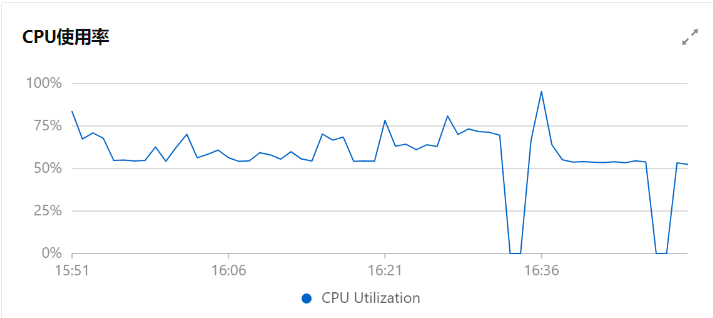
\includegraphics[width=0.45\textwidth]{./pic/continuous.png}
    \caption{Spark tasks are periodic tasks that are executed intermittently and have low load. After being attacked, viruses or mining programs usually occupy 50\% of the core, so the cpu utilization is stable at more than 50\%;}
    \label{fig:a-sec-cpu}
\end{figure}


\begin{figure}[H]
    \centering
    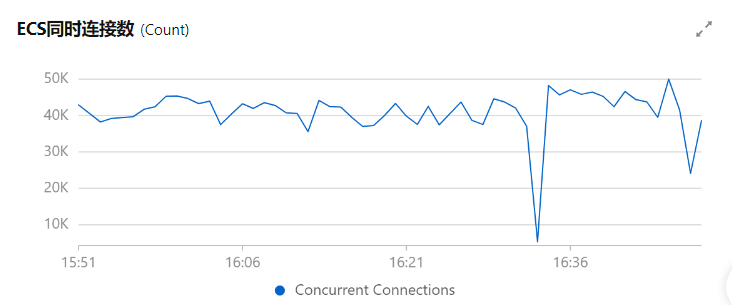
\includegraphics[width=0.45\textwidth]{./pic/cpu.png}
    \caption{Single normal user only has 20-30 ssh connections. After being attacked, the number of connections will soar to 40,000-50,000, resulting in almost unable to connect to the server to deal with the virus; The trough in the figure was caused by a server restart, after which the number of connections quickly recovered to more than 40,000}
    \label{fig:a-sec-ddos}
\end{figure}


\begin{figure}[H]
    \centering
    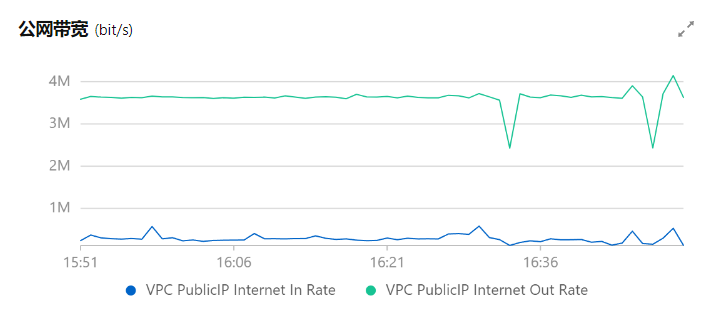
\includegraphics[width=0.45\textwidth]{./pic/ddos.png}
    \caption{Some mining viruses continue to generate data traffic in exchange for data}
    \label{fig:a-sec-bd}
\end{figure}


\begin{figure}[H]
    \centering
    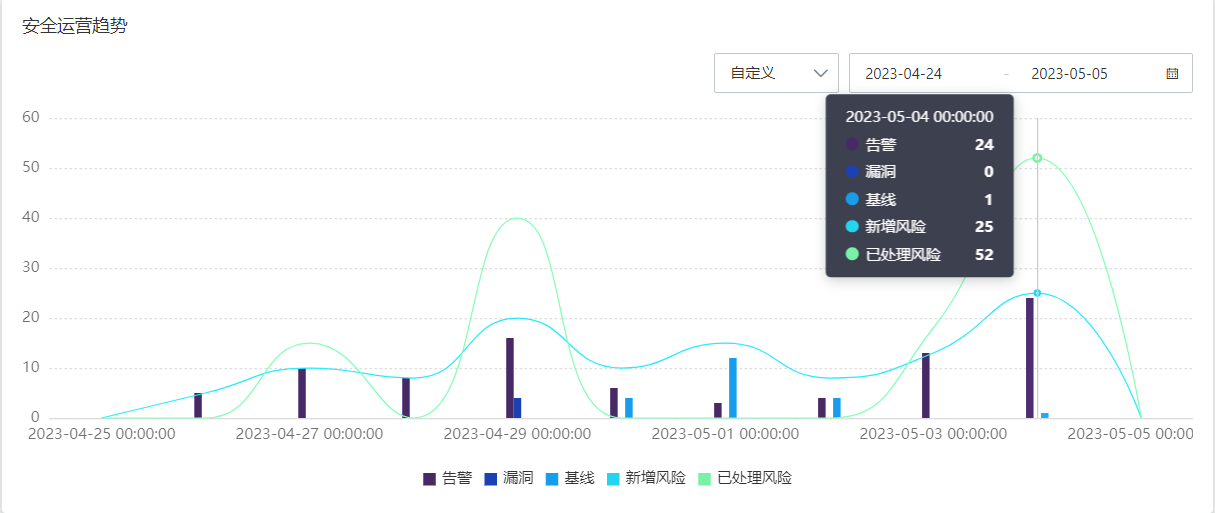
\includegraphics[width=0.5\textwidth]{./pic/secsta.png}
    \caption{Four servers in our cluster were sucessfully attacted every 12 hours. Each warning is a successful attack in the above figure.}
    \label{fig:a-sec-sta}
\end{figure}

On the presentation day of the project, which is 4th May, the server suffered the most serious intrusion, and the permission of MySQL stored key data was tampered, which resulted in the \textbf{loss of meta schema data of hive}. As a result, the data in the entire hdfs could not be properly identified. We had to delete all data collected, and recollect data again to complete the evening's presentation.